\chapter{Simulation Environment}

The Environment page defines the initial conditions and simulation time for the CFAST input file.

\begin{figure}[ht]
\centering
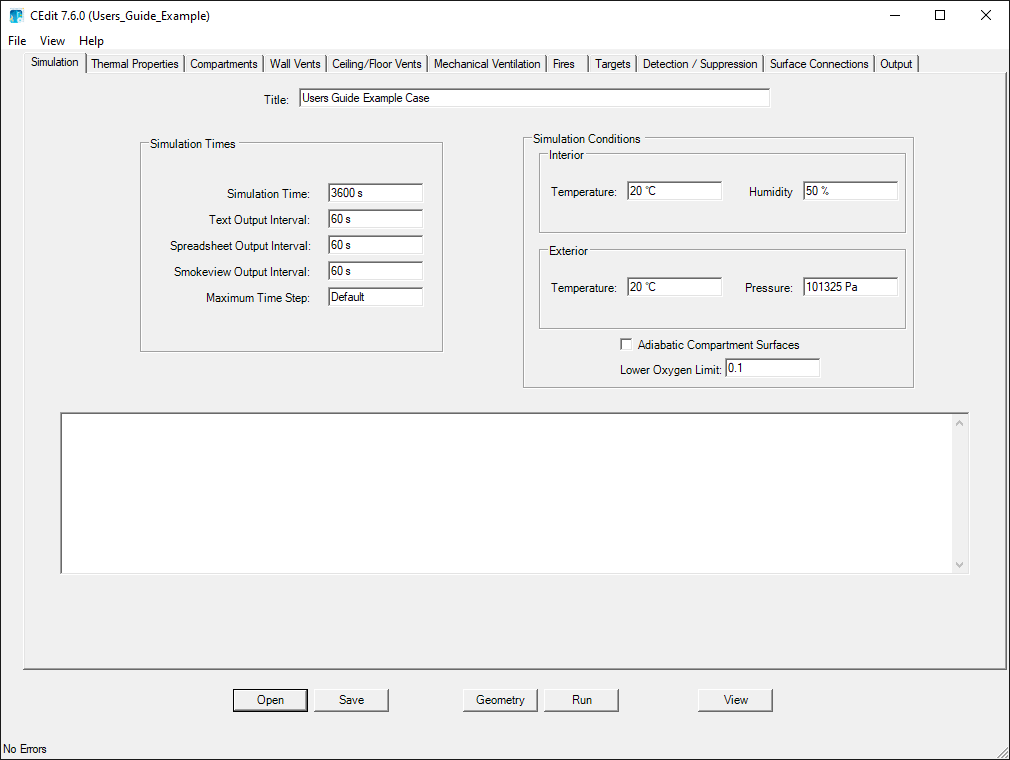
\includegraphics[width=6.5in]{FIGURES/Input_File/Environment_Tab}
\caption[The CFAST Simulation Environment Tab]{The CFAST Simulation Environment Tab.}
\end{figure}

\section{Title}

The first thing to do when setting up an input file is to give the simulation a title. The title is optional and may consist of letters, numbers, and/or symbols and may be up to 50 characters. All output files will be tagged with this character string.


\section{Simulation Times}

\begin{description}
\item[Simulation Time] (default units: s, default value, 900 s): The length of time over which the simulation takes place. The maximum value for this input is 86400 s (1 day).

\item[Text Output Interval] (default units: s, default value, 50 s): The time interval between each printing of the output data.  If omitted or less than or equal to zero, no output values will appear.

\item[Spreadsheet Output Interval] (default units: s, default value, 10 s): CFAST can output the results of the simulation in a comma-delimited spreadsheet file. This parameter defines the time interval between these outputs. A value greater than zero must be used if the spreadsheet file is desired.

\item[Smokeview Output Interval] (default units: s, default value: 10 s): CFAST can output a subset of the results in a format compatible with the visualization program Smokeview. This input defines the time interval between outputs of the model results in a Smokeview-compatible format.  A value greater than zero must be used if the Smokeview output is desired.

\item[Maximum Time Step] (default units: s, default value: 2 s): CFAST will automatically adjust the time interval for the solution of the differential equation set up or down so that the simulation is as efficient as possible within the pre-defined error tolerances. This parameter places a maximum value for the equation solver and can normally be left at the default value. In cases (which are hopefully rare) where the model fails to converge on a solution, this value can be reduced which often will allow the simulation to successfully complete.
\end{description}

\section{Ambient Conditions}

Ambient conditions define the environment at which the scenario begins. Initial pressures in a structure are calculated simply as a lapse rate (related to the height above sea level) based on the NOAA/NASA tables \cite{GPO:Atmosphere}. It is convenient to choose the base of a structure to be at zero height and then reference the height of the structure with respect to that height.  The temperature and pressure must then be measured at that position.  Another possible choice would be the pressure and temperature at sea level, with the structure elevations then given with respect to mean sea level.  This is also acceptable, but somewhat more tedious in specifying the construction of a structure.  Either of these choices works though, so long as they are consistent. Usually, the station elevation is set to zero and the pressure to ambient. The effect of changing these values is minor. Note that the equations implemented in the model are not designed to handle negative elevations and altitudes.

\begin{description}
\item[Temperature] (default units: \degc, default value: 20 \degc): Initial ambient temperature inside or outside the structure at the station elevation.

\item[Pressure] (default units: Pa, default value: 101300 Pa): Initial values for ambient atmospheric pressure inside and outside the structure at the station elevation. The default value is standard atmospheric pressure at sea level.

\item[Elevation] (defaults units: m, default value: 0 m): The height where the ambient pressure and temperature are specified.  This is the reference height for calculating the density of the atmosphere as well as the temperature and pressure inside and outside of the structure as a function of height.

\item[Humidity] (default units \% RH, default value: 50 \%): The initial relative humidity in the system, only specified for the interior.  This is converted to kilograms of water per cubic meter as an initial condition for both the interior and exterior of the structure.
\end{description}






\chapter{Compartments}

\begin{figure}[h!]
\begin{center}
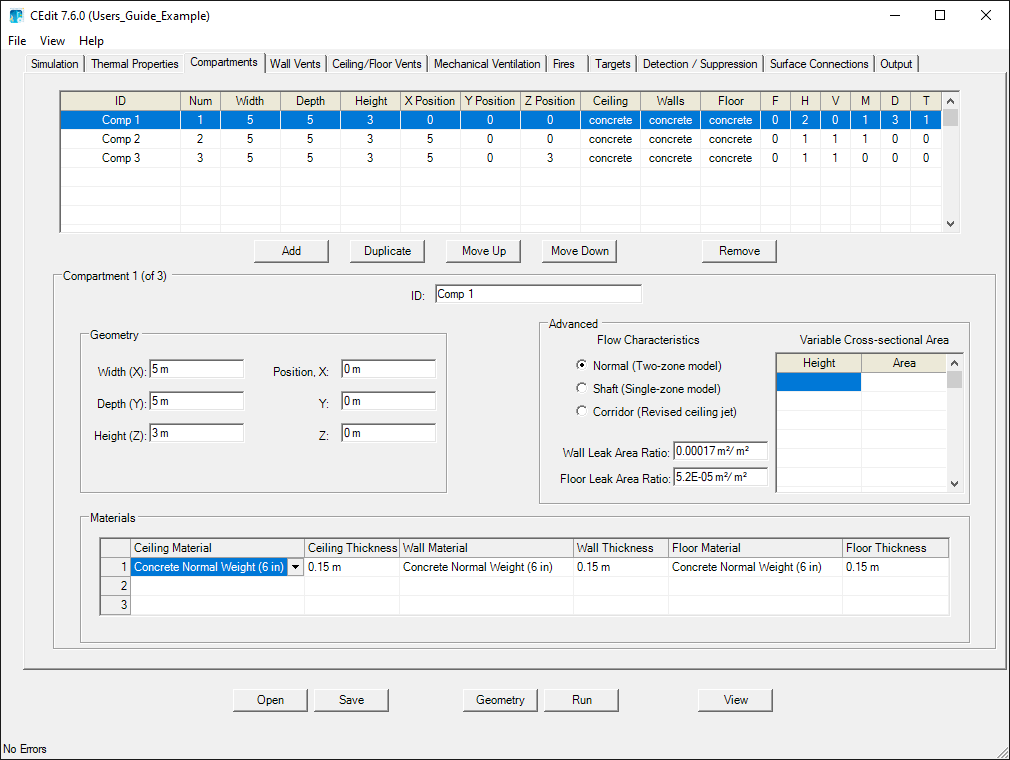
\includegraphics[width=6.5in]{FIGURES/Input_File/Compartment_Geometry_Tab}
\caption[The CFAST Compartments Tab]{The CFAST Compartments Tab.}
\end{center}
\end{figure}

The Compartments page defines the size, position, materials of construction, and flow characteristics for the compartments in the simulation. Initially, only the simulation environment page and the 'Add' button on the compartment geometry page is enabled; all other pages are not available to the user for detailed inputs until a compartment has been added to the simulation.

In order to model a fire scenario, the size and position of each compartment in the structure must be specified. For a compartment, the width, depth, compartment height and height of the floor of the compartment provide this specification. The maximum number of compartments for version 6 is thirty. The usual assumption is that compartments are rectangular parallelepipeds. However, the CFAST model can accommodate odd shapes as equivalent floor area parallelepipeds or with a cross-sectional area that varies with height.

\begin{figure}[h!]
\begin{tabular*}{\textwidth}{c@{\extracolsep{\fill}}c}
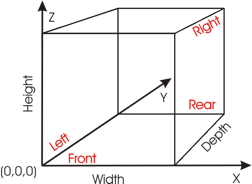
\includegraphics[width=2.5in]{FIGURES/Input_File/CFAST_Coordinates} &
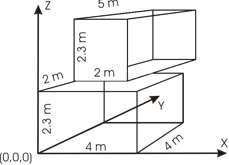
\includegraphics[width=2.6in]{FIGURES/Input_File/CFAST_Absolute_Positioning} \\
Compartment Size & Compartment Position
\end{tabular*}
\caption[Compartment Orientation and Positioning in CFAST]{Compartment Orientation and Positioning in CFAST.}
\label{fig:compartment_positioning}
\end{figure}

At least one compartment must be specified in the input file.  There are no defaults for compartment size. There are defaults for absolute positioning (0,0,0). The fully mixed (single zone) and corridor models are turned off by default.

\label{Compartment_Geometry}Compartments in CFAST are most typically defined by a width, depth, and height.  If desired, compartments can be prescribed by the cross-sectional area of the compartment as a function of height from floor to ceiling for other shapes. The absolute position of the compartment with respect to a single structure reference point can be defined to ease visualization or to allow exact placement of vents and surfaces relative to other compartments in a detailed calculation. This specification is important for positioning the compartments for visualization in Smokeview.

\begin{description}
\item[Compartment Name:] Compartments are identified by a unique alphanumeric name.  This may be a simple as a single character or number, or a description of the compartment.
\end{description}

\section{Geometry}

\label{Compartment_Inputs}
\begin{description}
\item[Width] specifies the width of the compartment as measured on the X axis from the origin (0,0,0) of the compartment.

\item[Depth] specifies the depth of the compartment as measured on the Y axis from the origin (0,0,0) of the compartment.

\item[Height] specifies the height of the compartment as measured on the Z axis from the origin (0,0,0) of the compartment.

\item[Absolute Width Position (Position X)] specifies the absolute x coordinate of the lower, left, front corner of the room.

\item[Absolute Depth Position (Position Y)] specifies the absolute y coordinate of the lower, left, front corner of the room.

\item[Absolute Floor Height (Position Z)] specifies the height of the floor of each compartment with respect to station elevation specified by the internal ambient conditions reference height parameter.  The reference point must be the same for all elevations in the input data.  For example, the two rooms in the sample to the right in figure~\ref{fig:compartment_positioning} would be located at (0,0,0) and (0,2,2.3).
\end{description}

\section{Materials}

To calculate heat loss through the ceiling, walls, and floor of a compartment, the properties of the bounding surfaces must be known. This includes the thermophysical properties of the surfaces and the arrangement of adjacent compartments if inter-compartment heat transfer is to be calculated.

The bounding surfaces are the ceilings, walls and floors that define a compartment. These are referred to as thermophysical boundaries, since each participates in conduction and radiation as well as defining the compartments, unless these phenomena are explicitly turned off.

The thermophysical properties of the surfaces which define compartments are described by specifying the thermal conductivity, specific heat, emissivity, density, and thickness of the enclosing surfaces for each material and then assigning the material to the ceiling, walls, and floor of a compartment.  Thermal properties for materials are read from the CFAST input file.  The thermophysical properties are specified at one condition of temperature, humidity, etc.  Only a single layer per boundary is allowed (some previous versions allowed up to three).

\begin{description}
\item[Ceiling Material] (default value: Gypsum Board): material name from the thermal properties data file used for the ceiling surface of the compartment.

\item[Wall Material] (default value: Gypsum Board): material name from the thermal properties data file used for the wall surfaces of the compartment.

\item[Floor Material] (default value: Off): material name from the thermal properties data file used for the floor surface of the compartment.
    \end{description}

\graybox{
If the thermophysical properties of the enclosing surfaces are not included, CFAST will treat them as adiabatic (no heat transfer). \\

If a name is used which is not in the input file, the model should stop with an error message. \\

The back surfaces of compartments are assumed to be exposed to ambient conditions unless specifically specified (see the section on Surface Connections) to specify heat transfer connections between compartments).
}

\section{Adding and Editing Thermal Properties}

By default, CEdit does not include predefined thermal properties for compartment materials. Thus, the user needs to define materials for use with a specific simulation.  These may be from other simulations or input directly from reference sources or test results. The \textbf{Edit, Thermal Properties, Insert Thermal Properties} Menu item allows you to add thermal properties from an existing data file to the current simulation.

\begin{figure}[h!]
\begin{center}
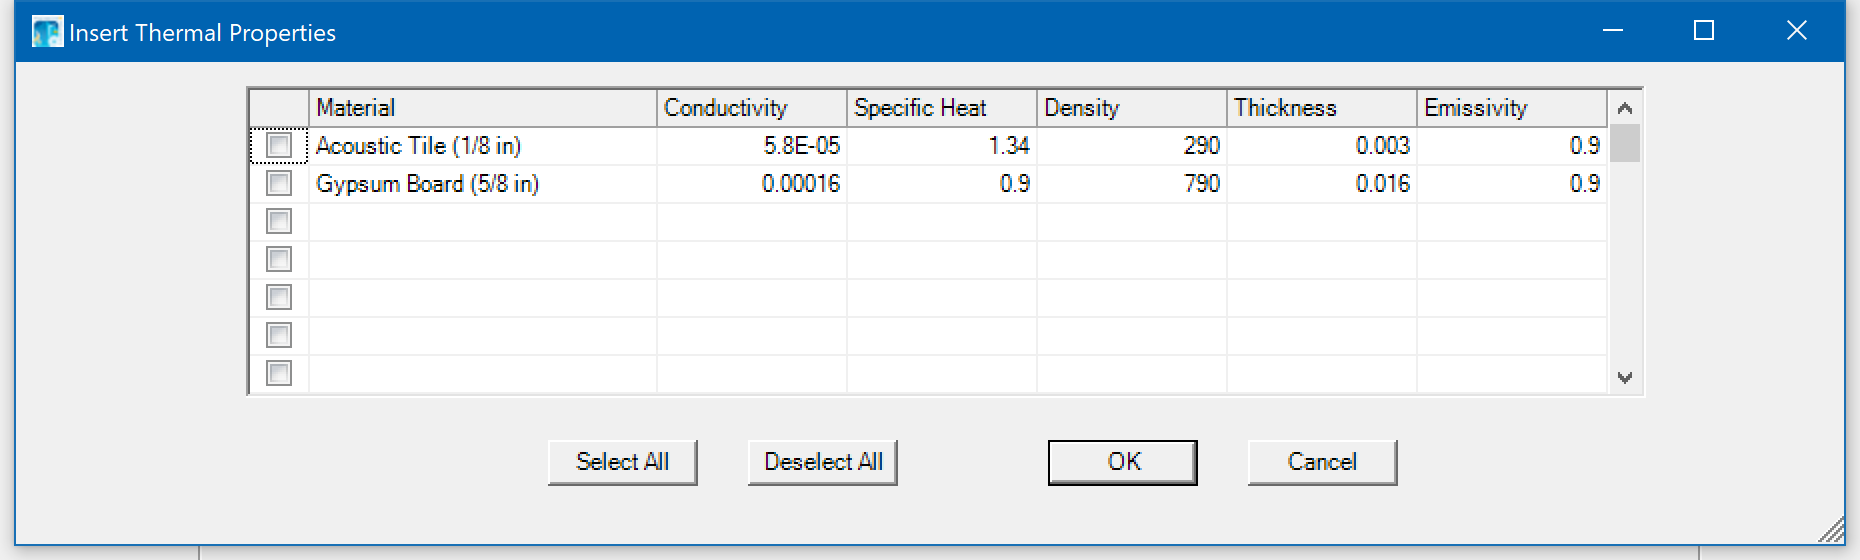
\includegraphics[width=6.5in]{FIGURES/Input_File/Insert_Thermal_Properties}
\caption[Inserting Thermal Properties in CFAST]{Inserting Thermal Properties in CFAST.}
\end{center}
\end{figure}

To add additional thermal properties to a simulation or to edit existing ones, the \textbf{Edit, Thermal Properties, Edit Thermal Properties} menu item allows you to edit any of the existing thermal properties.

\begin{figure}[h!]
\begin{center}
\includegraphics[width=6.5in]{FIGURES/Input_File/Edit_Thermal_Properties}
\caption[Editing Thermal Properties in CFAST]{Editing Thermal Properties in CFAST.}
\end{center}
\end{figure}

\begin{description}
\item[Material] A descriptive name for the material.

\item[Short Name] A one-word (no more than 8 characters) \textbf{unique} identifier for the material.  This identifier should not contain any spaces and is used in other CFAST inputs to identify the particular material referenced.

\item[Thermal Conductivity] (default value: none, default units: kW/m \degc): Thermal conductivity for the material.

\item[Specific Heat] (default value: none, default units: kJ/kg \degc): Specific heat for the material.

\item[Density] (default value: none, default units: kg/m$^3$): Density for the material.

\item[Thickness] (default value: none, default units: m): Thickness of the material.  Note that if two materials with identical thermal properties but with different thicknesses as desired, two separate materials must be defined.

\item[Emissivity] (default value: 0.9, default units: none): Emissivity of the material surface.  This is the fraction of radiation that is absorbed by the material.
\end{description}


\section{Modeling a Compartment as a Tall Shaft or Long Corridor}

For tall compartments or those removed from the room of fire origin, the compartment may be modeled as a single, well-mixed zone rather than the default two-zone assumption. A single zone approximation is appropriate for smoke flow far from a fire source, where the two-zone layer stratification is less pronounced than in compartments near the fire or in situations where the stratification does not occur. Examples are elevators, shafts, complex stairwells, or compartments far from the fire.

By specifying the compartment as a corridor, the ceiling jet temperature is calculated with a different empirical correlation that results in a somewhat higher temperature near the ceiling.  This will impact, for example, detectors, sprinkler, and targets near the ceiling in corridors.

\begin{description}
\item[Normal (Two-zone model)] Conditions in the compartment are calculated with the normal two-zone approach.

\item[Shaft (Single-zone model)] Conditions in the compartment are calculated as a single well-mixed zone.

\item[Corridor (Revised ceiling jet)] Conditions in the compartment are calculated with the normal two-zone approach. Ceiling jet temperatures in the compartment are calculated with a revised empirical correlation specific to corridors.
\end{description}


\section{Defining Variable Compartment Area}

The Compartment Geometry page includes two additional entries that may be used for defining compartment properties for spaces which are not rectangular in area.  Values for a chosen compartment are entered in a spreadsheet.

\begin{description}
\item[Height Value(s)] (default units: m, default values: none): Values of height for the corresponding cross-sectional area values measured from the floor of the compartment. The values for the compartment correspond to cross-sectional area values included for the same compartment on the ROOMA command.

\item[Area Value(s)] (default units m$^2$, default values: none): Values of cross-sectional area of the compartment as a function of height measured from the floor of the compartment. The values for the compartment correspond to height values included for the same compartment on the ROOMH command.
\end{description}

\graybox{
Cross-sectional area values may vary larger or smaller with height as appropriate. \\

Overall compartment size (input with the COMPA command (see page \pageref{Compartment_Inputs})) must define a volume at least as large as the total volume of the compartment. Typically, the COMPA input can correspond to the largest area in the list of cross-sectional area values. \\

Once the total compartment volume is determined from the set of cross-sectional area and height inputs, an effective width and depth are calculated (maintaining the original user input for compartment height) so the compartment volume matches the actual total volume of the compartment. The aspect ratio (width/depth) is maintained. \\

Cross-sectional area values should be input in order by ascending height. If the first height value is not zero (i.e., at floor level), the cross-sectional area is assumed constant from the floor to the height specified in the first cross-sectional area value. \\

Similarly, if the last height value is not at the ceiling height, the cross-sectional area is assumed constant from the height specified in the last cross-sectional area value to the ceiling.
Between any two adjacent cross-sectional area data values in the input list, the area is assumed to be a pyramidal section (which by definition maintains the same width to depth aspect ratio for the compartment from floor to ceiling). \\

CFAST uses the variable cross-sectional area inputs to determine the layer height. The equations solved by CFAST determine the volume of the upper layer. For a normal rectangular room, this corresponds directly to a layer height. For a variable cross-sectional area compartment, a  numerical integration of the area inputs beginning at the ceiling is used to determine the height at which the upper layer occupies the calculated volume of the upper layer.
}





\chapter{Natural Ventilation}

Natural ventilation can occur when two compartments are connected via open doorways or windows (\textbf{Wall Vents}); or when two compartments are connected via \textbf{Floor/Ceiling Vents}. If no vents are specified between two compartments, they are assumed to be isolated.

\section{Wall Vents}

\begin{figure}[h!]
\begin{center}
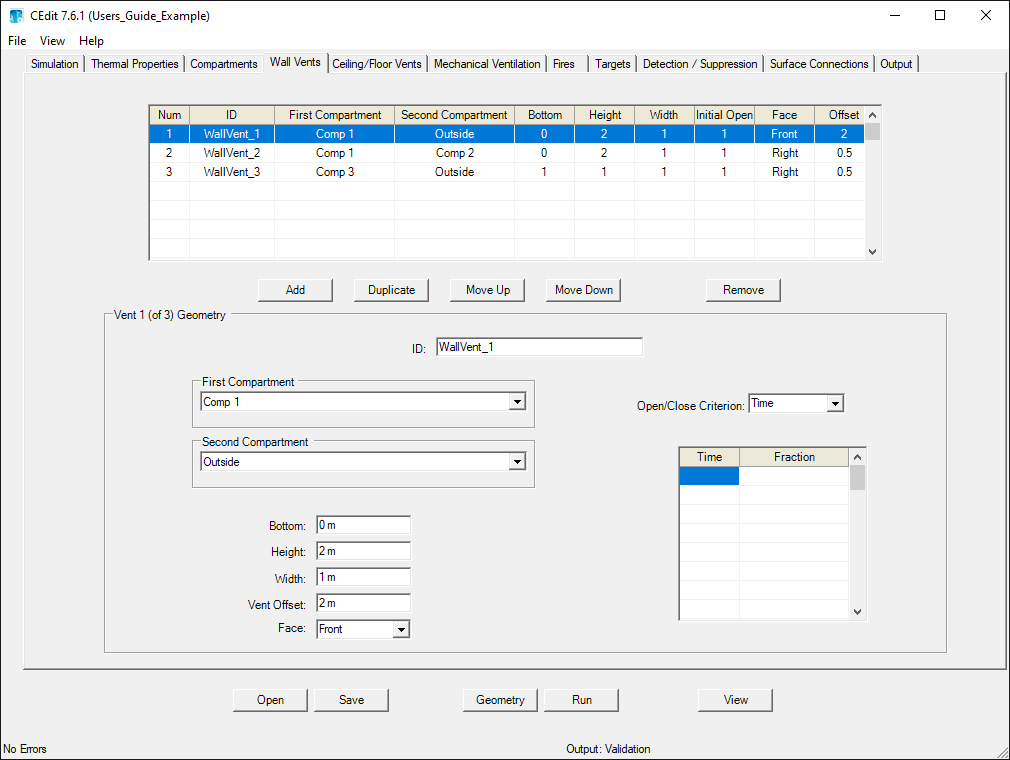
\includegraphics[width=6.5in]{FIGURES/Input_File/Natural_Flow_Tab}
\caption[The CFAST Wall Vents Tab]{The CFAST Wall Vents Tab.}
\end{center}
\end{figure}

Wall vents can only be created between compartments that physically overlap in elevation at some point. These may include doors between compartments or windows in the compartments (between compartments or to the outdoors).  Openings to the outside are included as openings to a compartment with a number one greater than the number of compartments described in the geometry section. It is possible to define a total of 25 horizontal flow connections between any pair of compartments. Horizontal flow connections may also be used to account for leakage between compartments or to the outdoors.

\begin{description}
\item[First Compartment] First of the two compartments to be connected by a horizontal flow vent.  Compartments are numbered automatically by the input editor and by the model in the order they are read from the input data file and/or the order they appear in the summary table on the compartment geometry page. Compartment numbers begin with 1, so the first compartment is number 1, the second 2, and so forth.

\item[Second Compartment] Second of the two compartments to be connected by a horizontal flow vent.

\item[Sill] (default units: m, default value: none): Sill height is the height of the bottom of the opening relative to the floor of the compartment selected as the first compartment.

\item[Soffit] (default units: m, default value: none): Position of the top of the opening relative to the floor of the compartment selected as the first compartment.

\item[Width] (default units: m, default value: none): The width of the opening.

\item[Initial Opening Fraction] (default value: 1): Flow through horizontal vents is calculated based on the area of the vent.  Normally, the vent is fully open.  If desired, the user may specify a fraction between 0 and 1 that allows the vent to be partially or fully closed at the beginning of the simulation.  In the model calculation, the vent width is multiplied by this fraction.  The opening fraction may be changed at any time in the simulation through the use of the EVENT command.

\item[Change Opening Fraction At Time]  (default units: s, default value: 0 s)  Time during the simulation at which to change the opening fraction.

\item[Final Opening Fraction] (default value: 1): for horizontal flow vents, the fraction specifies the fractional width opening of the vent. Fractional values must be between 0 and 1.

\item[Vent Offset] (default units: m, Default value: 0 m): For visualization, the vent offset is the horizontal distance between the near edge of this vent and the origin of the axis defined by the selected face (below) in the first compartment (Front and Rear are along the X-axis; left and right are along the Y-axis). For example, to place the vent at the center of the front wall, specify the front face at an offset of `compartment width/2 - vent width/2'.

\item[Face] For visualization, FACE specifies which wall the vent will be displayed on in Smokeview.  Choices are Front, Rear, Right, Left and are relative to the X-Z plane.
\end{description}

\graybox{
The soffit and sill specifications are with respect to the first compartment specified and are not necessarily symmetric since the elevation of the second compartment may be different than the first.  Reversing the order of the compartment designations can make a difference.
}

\section{Ceiling/Floor Vents}

\begin{figure}[h!]
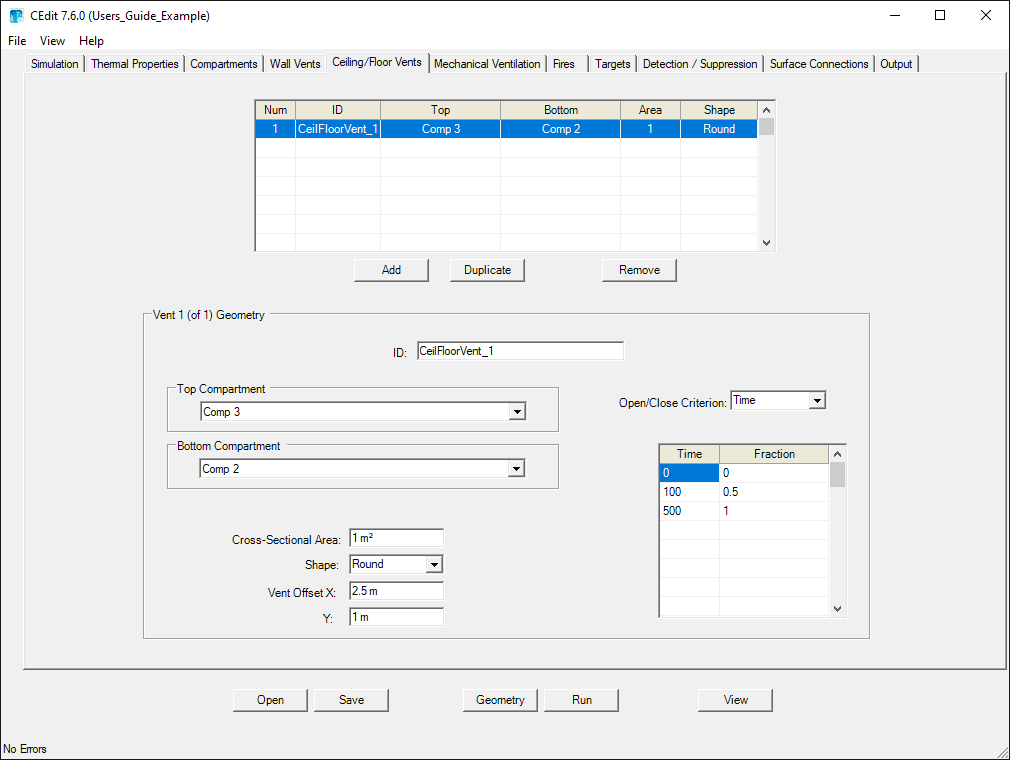
\includegraphics[width=6.5in]{FIGURES/Input_File/Vertical_Flow_Tab}
\caption[The CFAST Ceiling/Floor Vents Tab]{The CFAST Ceiling/Floor Vents Tab.}
\end{figure}

This section of the input data file describes the inputs for natural flow vents in ceilings and floors. Examples of these openings are scuddles in a ship, or a hole in the roof of a residence. Combined buoyancy- and pressure-driven flow through a vertical flow vent is possible when the connected spaces adjacent to the vent are filled with gases of different density in an unstable configuration, with the density of the top space larger than that of the bottom space. With a moderate cross-vent pressure difference, the instability leads to a bi-directional flow between the two spaces. For relatively large cross-vent pressure difference the flow through the vent is unidirectional, from the high- to the low-pressure space.

Connections can exist between compartments or between a compartment and the outdoors. Openings to the outside are included as openings to a compartment with a number one greater than the number of compartments defined in the scenario. There are four parameters which include each of the connected compartments, the shape of the opening, and the effective area of the vent.

\begin{description}
\item[Top Compartment] The top or first of the two compartments to be connected by a vertical flow vent. The vent is through the floor of this compartment.  Compartments are numbered automatically by the input editor and by the model in the order that they are read from the input data file and/or the order they appear in the summary table on the compartment geometry page. Compartment numbers begin with 1, so the first compartment is number 1, the second 2, and so forth.

\item[Bottom Compartment] The bottom or second of the two compartments to be connected by a horizontal flow vent.

\item[Cross-sectional Area] (default units: m$^2$, default value: none): specifies the cross-sectional area of the vent connecting the two compartments.

\item[Shape] The shape factor is 1 for circular openings and 2 for square openings. The shape factor changes the calculation of the effective diameter of the vent and flow coefficients for flow through the vent.

\item[Initial Opening Fraction] Flow through vertical vents is calculated based on the area of the vent.  Normally, the vent is fully open.  If desired, the user may specify a fraction between 0 and 1 that allows the vent to be partially or fully closed at the beginning of the simulation.  In the model calculation, the vent area is multiplied by this fraction.  The opening fraction may be changed at any time in the simulation through the use of the EVENT command.

\item[Change Opening Fraction At Time] (default units: s, default value: 0 s): Time during the simulation at which to change the opening fraction.

\item[Final Opening Fraction] for vertical flow vents, the fraction specifies the fractional cross-sectional area of the vent. Fractional values must be between 0 and 1.
\end{description}

\graybox{
Although obvious, note that the top or first compartment must be the compartment on top of the bottom or second compartment. \\

CFAST allows only a single connection between any pair of compartments included in a simulation. This limitation is based on the implementation of the vertical flow algorithm in CFAST and on the validation efforts for the original algorithm development  which only studied a single opening between connected compartments. \\

Vertical connections can only be created between compartments that could be physically stacked based on specified floor and ceiling elevations for the compartments.  Some overlap between the absolute floor height of one compartment and the absolute ceiling height of another compartment is allowed.  However, whether the compartments are stacked or overlap somewhat, the ceiling/floor absolute elevations must be within 0.01 m of each other. The check is not done when the connection is to the outside.
}





\chapter{Mechanical Ventilation}

\begin{figure}[h!]
\begin{center}
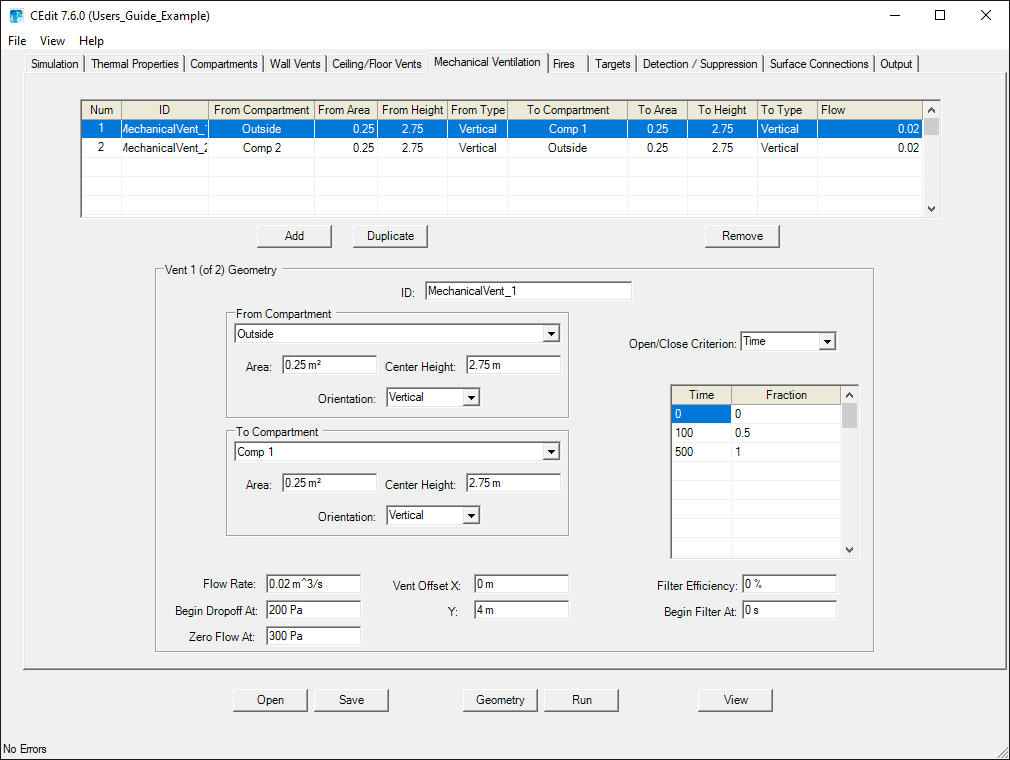
\includegraphics[width=6.5in]{FIGURES/Input_File/Mechanical_Vent_Tab}
\caption[The CFAST Mechanical Vents Tab]{The CFAST Mechanical Vents Tab.}
\end{center}
\end{figure}

Fan-duct systems are commonly used in buildings for heating, ventilation, air conditioning, pressurization, and exhaust. Generally, systems that maintain comfortable conditions have either one or two fans.  Residences often have a system with a single fan. Further information about these systems is presented in  Klote and Milke \cite{Klote:2002} and the American Society of Heating, Refrigerating and Air Conditioning Engineers Handbook \cite{ASHRAE:2001}.

The model for mechanical ventilation used in CFAST is based on the theory of networks and is based on the model developed by Klote \cite{Klote:1988a}.  This is a simplified form of Kirchoff's law which says that flow into a node must be balanced by flow out of the node. The equations used describe the relationship between the pressure drop across a duct, the resistance of a duct, and the mass flow.  The pressure can be changed by conditions in a compartment, or a fan in line in the duct system.  Resistance arises from the finite size of ducts, roughness on duct surfaces, bends and joints. In CFAST, default values are used for the duct properties, and thus mechanical ventilation connections are simply described by the connections to the two compartments and a fan whose throughput is a constant volumetric flow up to a user-specified pressure drop across the fan, dropping to zero at high backwards pressure on the fan.

\section{Connections to Compartments}

\begin{description}
\item[From Compartment] The first compartment to which the mechanical ventilation system diffuser is connected. Fan flow is from this compartment.  Compartments are numbered automatically by the input editor and by the model in the order they are read from the input data file and/or the order they appear in the summary table on the compartment geometry page. Compartment numbers begin with 1, so the first compartment is number 1, the second 2, and so forth.

\item[From Compartment Area] (default units: m$^2$, default value: none): Cross-sectional area of the opening into the compartment. The effective size of the vent is taken to be the square root of the area of the vent for the width and depth (vertically-oriented vents)/height (horizontally-oriented vents).

\item[From Compartment Height] (default units: m, default value: none): Height of the duct opening above the floor of the compartment measured from the floor to the midpoint of the diffuser.

\item[From Compartment Orientation] The orientation of the diffuser relative to the floor of the compartment.  A horizontal diffuser implies vertical flow through the ceiling or floor of the compartment.  A vertical diffuser implies horizontal flow through a wall of the compartment.

\item[To Compartment] The bottom or second of the two compartments to be connected by a horizontal flow vent. The vent is through the ceiling of this compartment.

\item[To Compartment Area] (default units: m$^2$, default value: none): Cross-sectional area of the opening into the compartment.

\item[To Compartment Height] (default units: m, default value: none): Height of the duct opening above the floor of the compartment measured from the midpoint of the diffuser.

\item[To Compartment Orientation] The orientation of the diffuser relative to the floor of the compartment.
\end{description}

\section{Fans}

\begin{description}
\item[Flow Rate] (default units: m$^3$/s, default value: none): Constant flow rate of the forced-air flow from the first compartment to the second compartment.

\item[Begin Drop Off Pressure] (default units: Pa, default value: 200 Pa): The description of the fan includes a drop off in flow beginning at a pressure specified by the user.  Above this pressure drop, the flow gradually drops to zero flow.

\item[Zero Flow Pressure] (default units: Pa, default value: 300 Pa): Specifies the pressure above which the flow through the mechanical ventilation connection is zero.

\item[Initial Opening Fraction] Flow through mechanical vents is calculated based on the area of the vent.  Normally, the vent is fully open.  If desired, the user may specify a fraction between 0 and 1 that allows the vent to be partially or fully closed at the beginning of the simulation.  In the model calculation, the fan flow rate is multiplied by this fraction.  The opening fraction may be changed at any time in the simulation through the use of the EVENT command.

\item[Change Opening Fraction At Time] (default units: s, default value: none): Time during the simulation at which to change the opening fraction.

\item[Final Opening Fraction] for mechanical flow vents, the fraction specifies the fractional fan flow rate for the vent. Fractional values must be between 0 and 1.
\end{description}

\graybox{
CFAST does not include provisions for reverse flow through a fan. Calibration for backward flow is not provided by fan manufacturers, so the equations incorporated in CFAST do not allow for such flow. The problem is simply that in this flow regime, the fan has stalled, and likely will soon fail. \\

For vertically-oriented vents, the height and width will be adjusted if the vent height is set such that the height plus or minus the effective height is above the compartment ceiling or below the floor. For example, a 1~m$^2$ vertically oriented vent placed only 0.2~m from the compartment floor will have an effective height of 0.7~m (0.5~m above the midpoint but limited to 0.2 m below the midpoint to the level of the compartment floor).
}

\section{Filtering}

For mechanical vents, there are two species that can be filtered out of the gas flow: soot and the user-defined trace species. Filters are applied only to fan openings. The fan must have been defined before the filter can be applied. Initially filtering is off. It is turned on with the EVENT key word, defined in the input editor with a Filter Efficiency and Begin Filter At time.

\begin{description}
\item[Filter Efficiency] (default units:~\%, default value: none): Flow through mechanical vents may include filtering that removes a user-specified portion of soot and trace species mass from the flow through the vent.  By default, there is no filtering applied, that is all of the soot and trace species mass in the vent flow is passed through the vent. Within the user interface, this is specified as a filter efficiency of 0~\%.  If desired, the user may specify the fraction of the soot and trace species mass to be removed as a percentage.

\item[Begin Filtering At Time] (default units: s, default value: none): Time during the simulation at which the mechanical vent filtering begins.
\end{description}

\graybox{
If the simulation includes mechanical ventilation filtering, care should be taken in choosing trace species production rates to insure the production rate is small compared to the total pyrolysis rate since the filtering removes mass from the system.  This will better allow appropriate conservation of mass in the solution of the system of differential equation.  For large production rates of trace species, scaling factors can be used (e.g., divide by 1000) for the trace species production rate to reduce the relative magnitude compared to the pyrolysis rate.  For analysis, the resulting trace species in compartments and filters can be converted back to original units multiplying by the scaling factor used.
}





\chapter{Fires}

A simulated fire in CFAST is implemented as a source of fuel mass which is released at a prescribed rate (the pyrolysis rate). Energy is released by the fuel and combustion products are created as it burns. In the fire, species production is calculated based on production yields prescribed by the user. In addition, the pyrolysis rate and resulting energy and species generation may be limited by the oxygen available for combustion. When sufficient oxygen is available for combustion, the heat release rate for the constrained fire is the same as for the unconstrained fire.

The model can simulate multiple fires in one or more compartments of the building.  These fires are treated as totally separate entities, with no interaction of the plumes. These fires are generally referred to as “objects” and can be ignited at a prescribed time, temperature or heat flux.

CFAST does not include a pyrolysis model to predict fire growth. Rather, pyrolysis rates for each fire are prescribed by the user.  While this approach does not directly account for increased pyrolysis due to radiative feedback from the flame or compartment, in theory these effects could be prescribed by the user as described in this section.  In an actual fire, this is an important consideration, and the specification used should consider the experimental conditions as closely as possible.

A fire releases energy based on the pyrolysis of fuel, but may be constrained by the oxygen available for combustion depending on the compartment conditions. Complete burning will take place only where there is sufficient oxygen.  When insufficient oxygen is entrained into the fire plume, unburned fuel will be transported from zone to zone until there is sufficient oxygen and a high enough temperature to support combustion.  In general, CFAST uses a simple definition of a combustion reaction that includes major products of combustion for hydrocarbon fuels:

\begin{eqnarray}
   \mathrm{C_{n_\C}H_{n_H}O_{n_O}N_{n_N}Cl_{n_{Cl}}} &+&  \nu_\OTWO \, \mathrm{O_2}  \rightarrow  \nonumber \\[.1in]
   \nu_\COTWO \, \mathrm{CO_2} &+& \nu_\HTWOO \, \mathrm{H_2O} \; + \; \nu_\CO \, \mathrm{CO} \; + \; \nu_\So \, \mathrm{Soot} \; + \; \nu_\HCl \mathrm{HCl} \; + \; \nu_\HCN \mathrm{HCN} \label{stoich}
\end{eqnarray} \\
assuming that all the nitrogen and chlorine in the fuel are converted to HCN and HCl. The stoichiometric coefficients $\nu_\So$, $\nu_\CO$, etc. represent appropriate molar ratios for a stoichiometric balance of the equation. For complete combustion of the simplest hydrocarbon fuel, methane reacts with oxygen to form carbon dioxide and water. The only inputs required are the fuel composition, heat release rate, and heat of combustion. For fuels that contain oxygen, nitrogen, or chlorine, the reaction becomes more complex. Stoichiometry is used to insure conservation of mass and elements in the reaction. The species which are calculated are oxygen, carbon dioxide, carbon monoxide, water, total unburned fuel (tuhc), and soot. Gaseous nitrogen is included, but only acts as a diluent.

\begin{figure}[h!]
\begin{center}
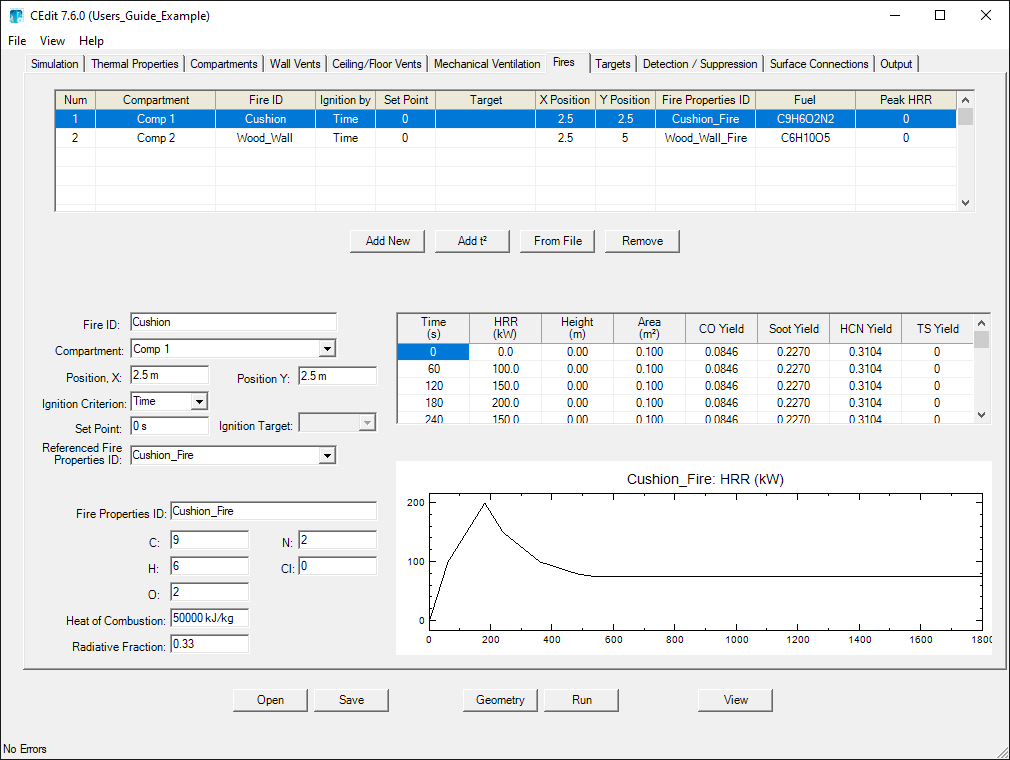
\includegraphics[width=6.5in]{FIGURES/Input_File/Fire_Tab}
\caption[The CFAST Fires Tab]{The CFAST Fires Tab.}
\end{center}
\end{figure}

Two inputs on the Fire Tab are global, that is, they apply to all fires included in a simulation.
\begin{description}
\item[Lower Oxygen Limit] (default units: \%, default value: 10~\%):  In the CFAST model, a limit is incorporated by limiting the burning rate as the oxygen level decreases until a ``lower oxygen limit'' (LOL) is reached. The lower oxygen limit is incorporated through a smooth decrease in the burning rate near the limit. Normally, this value would not be changed by the user.

\item[Gaseous Ignition Temperature] (default units: \degc, default value: ambient temperature plus 100 K): The lower temperature limit on the burning of fuel in a gas layer. Since CFAST does not support a combustion kinetics model, this is the algorithm used for fires out of vents.  Normally, this value would not be changed by the user.
\end{description}

\section{Defining Individual Fires}
\label{sec:fire_inputs}

Fires in CFAST are defined as a series of individual fire objects which are then placed as desired in compartments in a simulation.

Each fire object defines the time dependent variables of the fire described by the mass loss rate, rate of heat release, fuel height, and fuel area.  Species production rates are specified in a manner similar to the fire, entering the rates as a series of points with respect to time.  The species which are followed by CFAST are: carbon dioxide, carbon monoxide, hydrogen cyanide, hydrogen chloride, nitrogen, oxygen, soot, total unburned hydrocarbons and water. There is a separate calculation of the concentration-time product, typically denoted as Ct. Finally, a user-specified trace species can be specified to follow the transport that results from fire-induced flow for an arbitrary species. This may be of particular interest for radiological releases \cite{Jones:2008}, but may be useful for any trace amounts released by a fire.

Each fire object is defined in a separate comma-separated spreadsheet file with an extension of ``.o'' and is also saved in the CFAST input file for the current simulation. A pull-down menu allows the user to select one of the predefined fire objects to place in the chosen compartment. As many fire objects as desired may be defined by the user.  At least one fire in the simulation should ignite at a user-specified time.  Other fire objects can ignite based on time, temperature or heat flux conditions.

\begin{figure}[h!]
\begin{center}
\includegraphics[width=6.5in]{FIGURES/Input_File/Fire_Object_Edit}
\caption[Editing Fire Objects in CFAST]{Editing Fire Objects in CFAST.}
\end{center}
\end{figure}

\begin{description}
\item[Fire Object Name] The name for the desired object.  This also corresponds to the name of the fire object file, without the extension. The selected name must be unique (i.e., not the same as another fire object in the same simulation).

\item[Material] (default value: none): material name from the list of thermal properties used for the object. The material properties are used to calculate heat transfer into the object from its surroundings.

\item[C, H, O, N, Cl] Molecular formula of the burning fuel. Burning fuels in CFAST are assumed to be hydrocarbon fuels that contain at least Carbon and Hydrogen and optionally Oxygen, Nitrogen, and Chlorine. These five inputs define the stoichiometry of the fuel as it is burned.  Thus, for example, all of the specified Nitrogen and Chlorine is assumed to completely react to form HCN and HCl.  If only partial conversion is desired, a smaller ratio for Nitrogen and/or Chlorine can be specified.

\item[Heat of Combustion] (default units: J/kg, default value: 50 000 000 J/kg): The energy released per kilogram of mass burned.

\item[Soot Yield] (default units: kg/kg, default value: 0 kg/kg): Constant species yields of soot expressed as ratios of carbon to fuel produced by the pyrolysis of the fuel. This input allows the user to specify a single value for soot yield for all time points in the fire time line. Individual time points can be changed as desired in the spreadsheet input described below.

\item[CO Yield] (default units: kg/kg, default value: determined by correlation): Constant species yield of carbon monoxide expressed as a fraction of the fuel mass converted into carbon monoxide.  By default, the CO yield is related to the soot yield via the correlation developed by K\"oyl\"u and Faeth

\be
y_{CO} = \frac{12n_C}{M_fv_f}0.0014 + 0.37y_s \label{eq:Koylu}
\ee
where $n_C$ is the number of carbon atoms in a fuel molecule, $M_f$ is the molecular weight of the fuel, and $v_f$ is the stoichiometric coefficient of the fuel, assumed to be 1 here \cite{Koylu:1991}. Note that this correlation refers to well-ventilated fires. Yields of CO and soot in under-ventilated fires is still a subject of active research.

\item[Radiative Fraction] The fraction of the energy produced in combustion that is radiated from the fire and plume. Within CFAST, the radiative fraction defaults to 0.35 ; i.e., 35 \% of the fire’s energy is released via radiation.  For other fuels, the work of Tewarson \cite{Tewarson:2003}, McCaffrey \cite{McCaffrey:1982}, or Koseki \cite{Koseki:1989} is available for reference.  The typical range for the radiative fraction is from about 0.05 to 0.4.
\end{description}

For all fires, including t-squared fires, values are specified for time dependent variables, including default values for species generation. All of the time dependent variables depend on a predefined time line. The time input specifies a sequence of time points that define the timing of the fire.  An entry indicates a point on the time line when the mass loss rate, fuel height and other time dependent values are specified for the fire.  This time is independent of the simulation time which is specified by the TIMES line. Between specified time points, values for all time-dependent quantities are interpolated between adjacent specified values. If the simulation time is longer than the total duration of the fire, the final values specified for the fire (mass loss rate, fuel height, fuel area, and species production rates) are continued until the end of the simulation.

\begin{description}
\item[Time] (default units: s, default values: none): specify a sequence of time points that define the timing of the main fire.  An entry indicates a point on the time-line when the heat release rate, fuel height and other time dependent values are specified for the fire.

\item[Heat Release Rate (Qdot)] (default units: kW, default values: none): Heat release rate of the fire as a series of time points consistent with the time specification.

\item[Fire Height] (default units: m, default values: 0 m): Time-based values for height of the base of the fire.  The actual height of the base of the fire is the sum of the constant value specified for the fire and this time-varying height specification for a particular time in the fire development. Typically, only one of these two inputs will be used.

\item[Area] of the Base of the Fire (default units: m$^2$, default values: 0.3 m$^2$): Cross-sectional area of the base of the fire.

\item[CO Yield] (default units: kg/kg, default values: constant value from correlation, in eq. \ref{eq:Koylu}): yield of carbon monoxide expressed as a fraction of the fuel mass converted into carbon monoxide.

\item[Soot Yield] (default units kg/kg, default values: none): yield of soot expressed as a fraction of fuel mass converted into smoke particulate.

\item[Ct] (default units: none, default values: none): relative toxicity of combustion products produced by the fire.

\item[TS] (default units: kg/kg, default values: none): Yield of user-defined trace species per mass of fuel produced in the pyrolysis of the fuel.
\end{description}

\graybox{

Production of hydrogen cyanide and hydrogen chloride are tracked solely based on user prescribed yields. \\

The pyrolysis rate (and thus the heat release rate and species generation) for a fire may be reduced below its prescribed value based upon the oxygen available for combustion. \\

For a fire, the heat release rate is limited by available oxygen. This limit is applied in three places: The first is burning in the portion of the plume which is in the lower layer of the room of fire origin; the second is the portion of the plume in the upper layer, also in the room of origin; the third is in the vent flow which entrains air from a lower layer into an upper layer in an adjacent compartment. The unburned fuel is tracked in this model. Combustion of CO to CO$_2$ is not included in the model. Detailed combustion chemistry is not considered in CFAST due to the complexities associated with detailed kinetics and transport. \\

There are two calculations involving radiation in this model. One is for the overall energy balance and is based on broadband radiation absorption. The amount of radiation absorbed is sensitive to the species present, specifically water vapor, soot and carbon dioxide. The other is for visibility of egress signs. This calculation is based solely on the soot volume fraction and is reported as optical depth (per meter). The conversion factor is based on the recent work by Mulholland and Croarkin \cite{Mullholland:2000}. The conversion factor for converting mass density in kg/m$^3$ to optical depth is 3817 m$^2$/kg. The value reported is intended specifically for assessing the visibility of egress signs, based on the work of Jin \cite{Jin:1979}.  It is not applicable to the far blue or red regions of the spectrum and so should not be used for assessing optical detection of fires through smoke. \\

With the two parameters, heat of combustion ($H_C$) and heat release rate $\dQ$, the pyrolysis rate of the fuel is determined by $\dm=\frac{\dQ}{H_C}$. \\

By default, the fire is placed in the center of the compartment on the floor.  If values for any of the three position variables (x-position, y-position, z-position) are invalid (i.e., less than zero or greater than the compartment dimension in the appropriate direction), the location for that direction defaults to the center of the appropriate direction in the width or depth direction and at the floor for the vertical direction. \\

The area of the base of the fire should not be set to a value of zero. Radiation from the fire is determined by a point source calculation from the vertical center of the flame which is in turn determined by Heskestad's flame height correlation \cite{Heskestad:2002}, a function of heat release rate and fire area. \\

Ct represents the time-integrated exposure to the mass oncentration of all the mall of fuel consumed in a structure fire and is thus a concentration-time product (hence the name Ct). For ``normally toxic'' materials, Ct a value of 1 \cite{Levin:1982} has been recommended and is typically changed by an order of magnitude for particularly toxic or non-toxic materials.  It is not part of the mass balance for the fuel and system, but it carried along as a transported species in flow through the structure. Ct is used as a measure of toxicity of a material.  Typically the integrated Ct versus time product is calculated. For normal materials, a concentration-time product of 900 mg min/m$^3$ is an indication of incapacitation \cite{Levin:1982}. \\

The trace species TS is transported along with fire gases, but is assumed not to take part in the combustion reaction and is assumed not to be a significant source of overall mass for the system mass balance calculated by the model. This implies that the production rate of trace species specified should be much smaller than the total specified pyrolysis rate. If necessary, the trace species can be scaled to a smaller value (e.g., divided by 1000) for the simulation and converted back for analysis (e.g., multiplied by 1000). \\

In the input editor, time-dependent data are entered in a simple spreadsheet. Normal windows copy (Ctrl-C), cut (Ctrl-X), and paste (Ctrl-V) keyboard shortcuts are available for data editing. In addition, Alt-Ins will insert a complete row above the currently-selected row in the spreadsheet and Alt-Del will delete the current row in the spreadsheet.
}

\subsection{Adding and Editing Fires}

By default, CEdit does not include predefined fires. Thus, the user needs to define fire objects for use with a specific simulation.  These may be from other simulations or input directly from reference sources or test results. The \textbf{Edit, Fires, Insert Fires} Menu item allows you to add fires from an existing data file to the current simulation.

\begin{figure}[h!]
\begin{center}
\includegraphics[width=6.5in]{FIGURES/Input_File/Insert_Fire_Objects}
\caption[Inserting Fires in CFAST]{Inserting Fires in CFAST.}
\end{center}
\end{figure}

\subsection{T-squared Fires}

Use the Create t$^2$ button to create a new fire object with a heat release rate specified by the user in the form of a t-squared fire.  For a wide range of fires, the fire growth can be accurately represented with a power law relation of the form $\dQ=\alpha t^2$  where $\dQ$  is the heat release rate of the fire, $\alpha$ is the fire intensity coefficient, and $t$ is time \cite{Schifiliti:2002}. A set of specific t-squared fires labeled slow, medium, and fast, with fire intensity coefficients ($\alpha$) such that the fires reached 1054 kW (1000~BTU/s) in 600~s, 300~s, and 150~s, respectively were proposed for design of fire detection systems .  Later, these specific growth curves and a fourth called "Ultra-fast" which reaches 1054~kW in 75~s, gained favor in general fire protection applications. A separate window allows the user to define the t-squared fire. Details of the inputs for a t-squared fire is included below.

\begin{figure}[h!]
\begin{center}
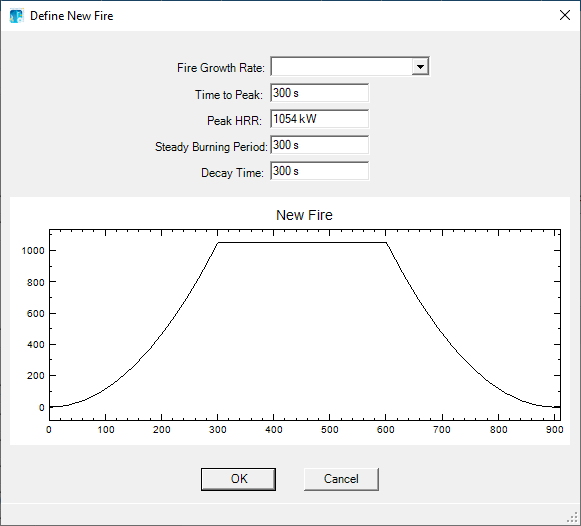
\includegraphics[width=5in]{FIGURES/Input_File/Create_t2}
\caption[Inserting T-squared Fires in CFAST]{Inserting T-squared Fires in CFAST.}
\end{center}
\end{figure}

\begin{description}
\item[Fire Growth Rate] A set of specific t-squared fires labeled slow, medium, fast, or ultra-fast with fire intensity coefficients ($\alpha$) such that the fires reached 1054~kW (1000~BTU/s) in 600~s, 300~s, 150~s, and 75~s are available.  Each of these growth rates (with corresponding decay rates) can be selected. A fifth, custom, selection allows the user to define any growth or decay rate desired.

\item[Time to Peak] (default units: s, default value: 300 s): The time for the fire to reach the peak fire size.

\item[Peak HRR] (default units: kW, default value: 1054 kW): The peak heat release rate of the t-squared fire.  Fire size is constant beginning at a time consistent with the time to reach the peak value,   and continues at that value for the time specified in the steady burning period, below.

\item[Steady Burning Period] (default units: s, default value: 300 s): Duration of time that the fire continues burning at the rate specified by the maximum HRR input, above.

\item[Decay Period] (default units: s, default value, 300 s): Duration of time for the fire to decay back to a zero value.  Decay follows the inverse of the t-squared growth rate.
\end{description}

\section{Fire Location}

Fires  are placed in defined positions within a compartment of a simulation and oriented with a normal vector to the surface of the object.  Ignition of an object may be at a specified time, a specified net incident heat flux on the surface of the object, or at a specified surface temperature of the object.

\begin{description}
\item[Compartment] of Fire Origin: specifies the compartment that contains the main fire for the simulation.  Any compartment defined is valid.

\item[Position X] (default units: m, default value: compartment width / 2): Position of the center of the base of the fire measured in the x direction from the front lower left corner of the compartment origin (0,0,0) in the compartment of fire origin.

\item[Position Y] (default units: m, default value: compartment depth / 2): Position of the center of the base of the fire measured in the y direction from the front lower left corner of the compartment origin (0,0,0) in the compartment of fire origin.

\item[Position Z] (default units: m, default value: 0 m): Position of the center of the base of the fire measured in the z direction from the front lower left corner of the compartment origin (0,0,0) in the compartment of fire origin. The actual height of the base of the fire is the sum of this constant value and the time-varying height specification for a particular time in the fire development. Typically, only one of these two inputs will be used.

\item[Normal  X] Component: specifies a vector of unit length perpendicular to the exposed surface of the object. The X component is in the direction from the rear wall of the object compartment. Default value is a horizontal, upward facing object, unit vector = (0,0,1)

\item[Normal  Y] Component: specifies a vector of unit length perpendicular to the exposed surface of the object. The Y component is in the direction from the left wall of the object compartment.

\item[Normal  Z] Component: specifies a vector of unit length perpendicular to the exposed surface of the object. The Z component is in the direction from the floor of the object compartment.

\item[Ignition Criterion] The type of ignition condition. Acceptable values are 1 for time, 2 for object surface temperature, and 3 for incident flux to object surface.

\item[Ignition Value] The numerical value at which ignition will occur. If it is less than or equal to zero, the default value of zero is taken.
\end{description}

\section{Calculating Normal Vectors}

Normal vectors are used to determine the orientation of the front face of fires and targets in CFAST in relations to other fires and compartment surfaces. This effects the heat flux to targets calculated by CFAST. The general equations for determining the normal vectors in the x, y, and z directions are \\~

Normal vector in the x direction, $x = \sfrac{x}{\sqrt{x^2 + y^2 + z^2}}$ \\

Normal vector in the y direction, $y = \sfrac{y}{\sqrt{x^2 + y^2 + z^2}}$ \\

Normal vector in the z direction, $z = \sfrac{z}{\sqrt{x^2 + y^2 + z^2}}$ \\
where $x$, $y$, and $z$ are distance from the surface of interest to a chosen reference point within the same compartment.

The simplest way to calculate the unit vector is to draw an imaginary line at right angles (i.e., 90$^\circ$ angle) from the exposed surface of the target and to extend this imaginary line until it hits the walls, floor or ceiling of the compartment in which it is located.  This imaginary line is actually a vector that starts at the front surface of a target and terminates on a wall, floor, or ceiling.  Once the start point and the end point of a vector are known, the unit vector for this imaginary line may be calculated as follows:

\begin{equation}
  \begin{aligned}
 x &= \sfrac{\brackets{x_{end} - x_{start}}}{\sqrt{\brackets{x_{end} - x_{start}}^2 + \brackets{y_{end} - y_{start}}^2 + \brackets{z_{end} - z_{start}}^2}} \\
 y &= \sfrac{\brackets{y_{end} - y_{start}}}{\sqrt{\brackets{x_{end} - x_{start}}^2 + \brackets{y_{end} - y_{start}}^2 + \brackets{z_{end} - z_{start}}^2}} \\
 z &= \sfrac{\brackets{z_{end} - z_{start}}}{\sqrt{\brackets{x_{end} - x_{start}}^2 + \brackets{y_{end} - y_{start}}^2 + \brackets{z_{end} - z_{start}}^2}}
  \end{aligned}
\end{equation}

As an example, assume the following scenario:

\begin{itemize}
\item A square shaped target object is located in the middle of the floor of a compartment.
\item The target is constructed from non-combustible materials except the top.
\item The square shaped material is 1 m in depth, 1 m in breadth, and 1 m high.
\item The reference point (0,0,0) in the compartment is the lower left hand side of the rear wall.
\item The compartment is 3 meters in the x direction (i.e., the distance from the rear wall to the front wall of the compartment), 4 meters in the y direction (i.e., the distance from the left wall to the right wall of the compartment), and 5 meters in the z direction (i.e., the distance from the floor to the ceiling of the compartment).
\end{itemize}

Since the only side of the target that is combustible is the top surface of the target object, an imaginary line is draw perpendicular (i.e., at a 90$^\circ$ angle) from the top surface of the target object and extended until it reaches the outer boundary of the compartment.  In this case, since the top of the target object is facing the ceiling, the imaginary line would run straight up to the ceiling, running parallel to the four walls of the compartment, and terminating at the ceiling at the point (1.5 m, 2 m, 5 m).  Since the vector starts at point (1.5-m, 2-m, 1-m) and terminates at (1.5-m, 2-m, 5-m), the unit vectors can be calculated as follows:


\begin{equation}
  \begin{aligned}
 x &= \sfrac{\brackets{x_{end} - x_{start}}}{\sqrt{\brackets{x_{end} - x_{start}}^2 + \brackets{y_{end} - y_{start}}^2 + \brackets{z_{end} - z_{start}}^2}} \\
 &= \sfrac{\brackets{1.5 - 1.5}}{\sqrt{\brackets{1.5 - 1.5}^2 + \brackets{2 - 2}^2 + \brackets{5 - 1}^2}} \\
 &= 0\\
 y &= \sfrac{\brackets{y_{end} - y_{start}}}{\sqrt{\brackets{x_{end} - x_{start}}^2 + \brackets{y_{end} - y_{start}}^2 + \brackets{z_{end} - z_{start}}^2}} \\
 &= \sfrac{\brackets{2 - 2}}{\sqrt{\brackets{1.5 - 1.5}^2 + \brackets{2 - 2}^2 + \brackets{5 - 1}^2}} \\
 &= 0 \\
 z &= \sfrac{\brackets{z_{end} - z_{start}}}{\sqrt{\brackets{x_{end} - x_{start}}^2 + \brackets{y_{end} - y_{start}}^2 + \brackets{z_{end} - z_{start}}^2}} \\
 &= \sfrac{\brackets{5 - 1}}{\sqrt{\brackets{1.5 - 1.5}^2 + \brackets{2 - 2}^2 + \brackets{5 - 1}^2}} \\
 &= 1\\
  \end{aligned}
\end{equation}

In this case, the unit vector in the +Z direction.





\chapter{Sprinklers and Detectors}

Sprinklers and detectors are both considered detection devices by the CFAST model and are handled using the same inputs.  Detection is based upon heat transfer to the detector. Fire suppression by a user-specified water spray begins once the associated detection device is activated.

\begin{figure}[h!]
\begin{center}
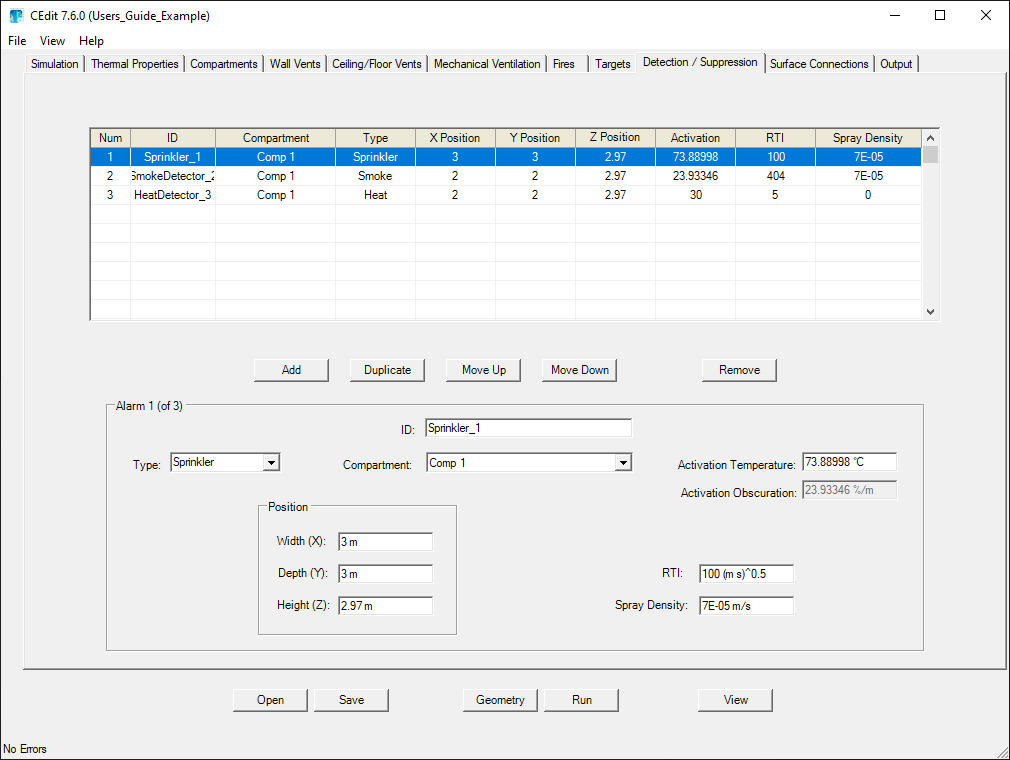
\includegraphics[width=6.5in]{FIGURES/Input_File/Detector_Tab}
\caption[The CFAST Detection/Suppression Tab]{The CFAST Detection/Suppression Tab.}
\end{center}
\end{figure}

\begin{description}
\item[Type] type of detector, select smoke detector, heat detector, or sprinkler.

\item[Compartment] the compartment in which the detector or sprinkler is located.

\item[Activation Temperature] (default units: \degc, default value: dependent on type): the temperature at or above which the detector link activates.

\item[Width (X)] Position (default units: m, default value: none): position of the object as a distance from the left wall of the compartment (X direction).

\item[Depth (Y)] Position (default units: m, default value: none): position of the detector or sprinkler as a distance from the front wall of the compartment (Y direction).

\item[Height (Z)] Position (default units: m, default value: none): position of the object as a distance from the floor of the compartment (Z direction).

\item[RTI] (default units: (m$\cdot$s)$^{1/2}$, default value: none): the Response Time Index (RTI) for the sprinkler or detection device.

\item[Spray Density] (default units: m/s, default value: none): the amount of water dispersed by a sprinkler.  The units for spray density are length/time, derived by dividing the volumetric flow rate by the spray area. The suppression calculation is based upon an experimental correlation by Evans~\cite{Evans:1993}.
\end{description}

\graybox{
Often, the activation of smoke alarms is simulated with a temperature-based criterion, typically in the range of 5~\degc to 10~\degc above ambient. Davis and Notarianni  studied the activation of heat and smoke alarms in small and large compartments \cite{Davis:1996}. They conclude that a temperature rise of approximately 5~\degc corresponded to activation of ionization alarms for a range of fire sources and ceiling heights. The Nuclear Regulatory Commission includes a default value of 10~\degc in NUREG-1805 \cite{NRCNUREG1805}. \\

Several cautions should be observed when using estimates of sprinkler suppression within the model: 1)~The first sprinkler activated controls the effect of the sprinkler on the heat release rate of the fire.  Subsequent sprinklers which may activate have no additional effect on the fire simulation. 2)~The fire suppression algorithm assumes the effect of the sprinkler is solely to reduce the heat release rate of the fire. Any effects of the sprinkler spray on gas temperatures or mixing within the compartment are ignored. 3)~The sprinkler always reduces the heat release rate of the fire. The ability of a fire to overwhelm an under-designed sprinkler is not modeled. 4) Since the dynamics of the sprinkler and direct effects of the spray on gas temperatures and velocities are not modeled, calculated times of activation of secondary sprinklers and / or detectors after the first sprinkler is activated should be not be modeled since the impact of the first sprinkler on the activation of additional sprinklers is not included in the CFAST model.
}



\chapter{Defining Targets}

CFAST can track and report calculations of the net heat flux striking arbitrarily positioned and oriented targets and the temperature of these targets.

\begin{figure}[h!]
\begin{center}
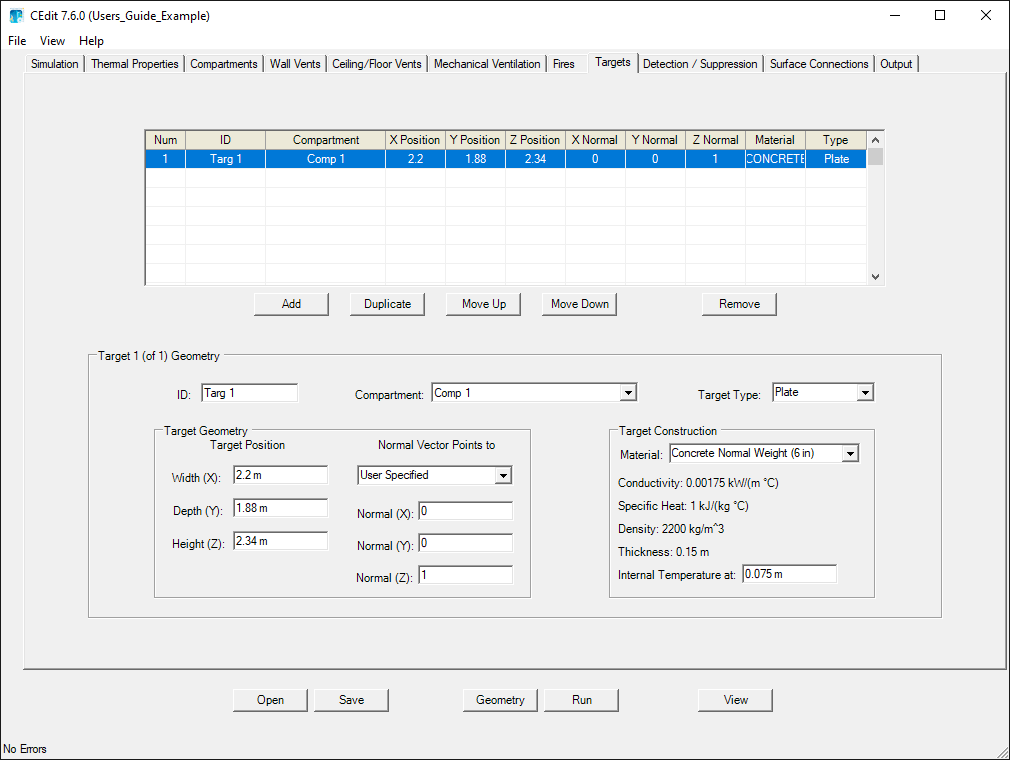
\includegraphics[width=6.5in]{FIGURES/Input_File/Target_Tab}
\caption[The CFAST Targets Tab]{The CFAST Targets Tab.}
\end{center}
\end{figure}

In addition to any user-defined targets, there are always two targets that are automatically placed in any compartment containing a fire. Both are included for reporting purposes. The first is an “ambient target” and is intended to represent the net flux to a human body. This is used for the flux in the hazard calculation for tenability. The assumption is that the target will remain at ambient temperature, which is a surrogate for body temperature. The second determines the net flux to a horizontal target on the floor whose temperature is assumed to be the same as the floor surface. The calculation can be used to estimate the ignition of combustibles on the floor as a surrogate for estimating time to flashover, typically taken to be 20 kW/m$^2$. Thus if user-specified targets are included, they will be in addition to these two predefined targets.

For all targets, heat flux is calculated to the surface specified by the user (with the direction determined by the normal vector). Conduction into the target is assumed to occur only from this surface into the target.

\begin{description}
\item[Compartment] The compartment in which the target is located.

\item[Target Type] If the solution method is not STEADY, this parameter further indicates the solutions equations.  Specify Thermally Thick, Thermally Thin, or Cylindrical.  For thermally thin materials, CFAST uses ordinary differential equations; for thermally thick materials, partial differential equations, and for cylindrical targets, partial differential equations in cylindrical coordinates.

\item[Solution Method] Optional parameter that indicates the solution method. STEADY for steady state solution, EXPLICIT for explicit solution, IMPLICIT for implicit solution.

\item[Width (X)] Position (default units: m, default value: none): Position of the target as a distance from the left wall of the target compartment (X direction).

\item[Depth (Y)] Position (default units: m, default value: none): Position of the target as a distance from the front wall of the target compartment (Y direction).

\item[Height (Z)] Position (default units: m, default value: none): Height of the target above the floor (Z direction).

\item[Normal Vector X] Component: specifies a vector of unit length perpendicular to the exposed surface of the target. (Width) component in the direction from the left wall of the target compartment. A value of 1 defines a vertical target facing into the compartment, unit vector = (1,0,0). The X, Y, and Z component of the normal vector can also be calculated automatically with a pull down menu that allows selection of surfaces and fires in the compartment visible from the target location.

\item[Normal Vector Y] Component: specifies a vector of unit length perpendicular to the exposed surface of the target. (Depth) component in the direction from the front wall of the target compartment. A value of 1 defines a vertical target facing to the right, unit vector = (0,1,0).

\item[Normal Vector Z] Component: specifies a vector of unit length perpendicular to the exposed surface of the target. (Height) component in the direction from the floor of the target compartment. Default value is a horizontal, upward facing target, unit vector = (0,0,1).

\item[Material] Used to specify the thermal properties of the target.  Any existing material in the list of thermal properties may be used here.

\item[Internal Temperature at] (default units: none, default value: 0.5): For each target, CFAST calculates the internal temperature at a number of node points within the target. By default, the reported internal temperature (in the printed and spreadsheet output) is the temperature at the center of the target, e.g., equidistant from the front and back faces of the target. This input allows the user to override this default position. The input represents the position as a fraction of the thickness from the front surface to the back surface of the material.
\end{description}

\graybox{
Target inputs in CFAST perform a heat transfer calculation between the compartment and the target. The steady state option assumes that the target material reacts instantly to changing conditions and computes the target temperature that would result in a balance of incoming and outgoing heat (i.e., a steady state). If a transient target temperature is modeled, then one can either assume that there is a temperature variation within the target or assume that the target is “thermally thin” and can be modeled using only one temperature. If the target is thermally thick, the numerical solution can be solved using an explicit or an implicit method.  Typically, the implicit method will work in all cases.  The explicit method is recommended only when the implicit method fails to come to a solution.
}





\chapter{Surface Connections}

\begin{figure}[h!]
\begin{center}
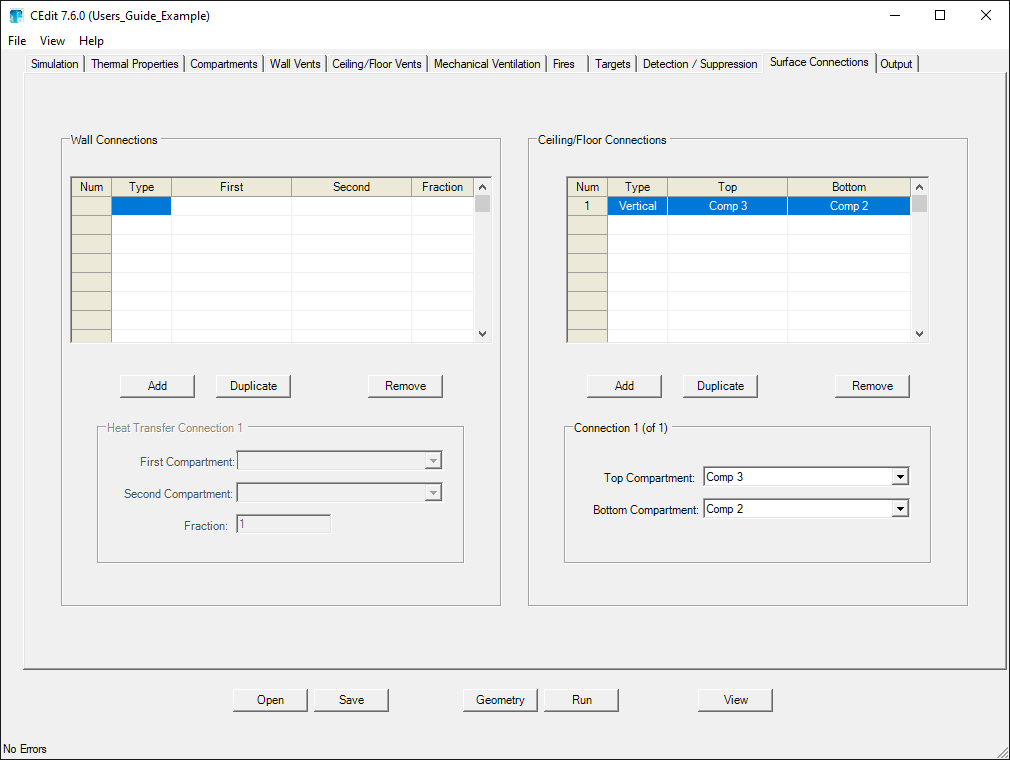
\includegraphics[width=6.5in]{FIGURES/Input_File/Surface_Connection_Tab}
\caption[The CFAST Surface Connections Tab]{The CFAST Surface Connections Tab.}
\end{center}
\end{figure}

The Surface Connections page allows the user to define heat transfer between compartments in a simulation. Energy can be transferred from compartment to compartment through solid boundaries (walls, ceilings and floors) by means of conduction. The heat transfer between connected compartments is modeled by setting the boundary condition for the outside surface of a compartment to the temperature of the outside surface of the  connected compartment.   As before, temperatures are determined by the solver so that the heat flux striking the wall surface (both interior and exterior) is consistent with the temperature gradient at that surface.

\begin{description}
\item[First Compartment] First of the connected compartments. Order of the inputs is not important.

\item[Second Compartment] Second of the connected compartments. Order of the inputs is not important.

\item[Fraction] Specifies the fraction of the vertical surface areas of the compartments which are connected can be specified. The fraction specifies the fraction of the vertical surface area connecting the first and second compartment pair.

\item[Top Compartment] The top or first of the two compartments to be connected by a vertical heat transfer connection. The connection is through the floor of this compartment.

\item[Bottom Compartment] The bottom or second of the two compartments to be connected by a vertical heat transfer connection. The connection is through the ceiling of this compartment.
\end{description}





\chapter{Visualization}

Calculated results from a CFAST simulation can be visualized using Smokeview \cite{Smokeview_Users_Guide_6}. This allows the user to see the compartment geometry and connections or view the results of the simulation visually. In addition to a simplified view of the layer temperatures and vent flows, more detailed estimates of gas temperature, gas velocity, vent flow velocity, target temperature, and detector status can be visualized.

\begin{figure}[h!]
\begin{center}
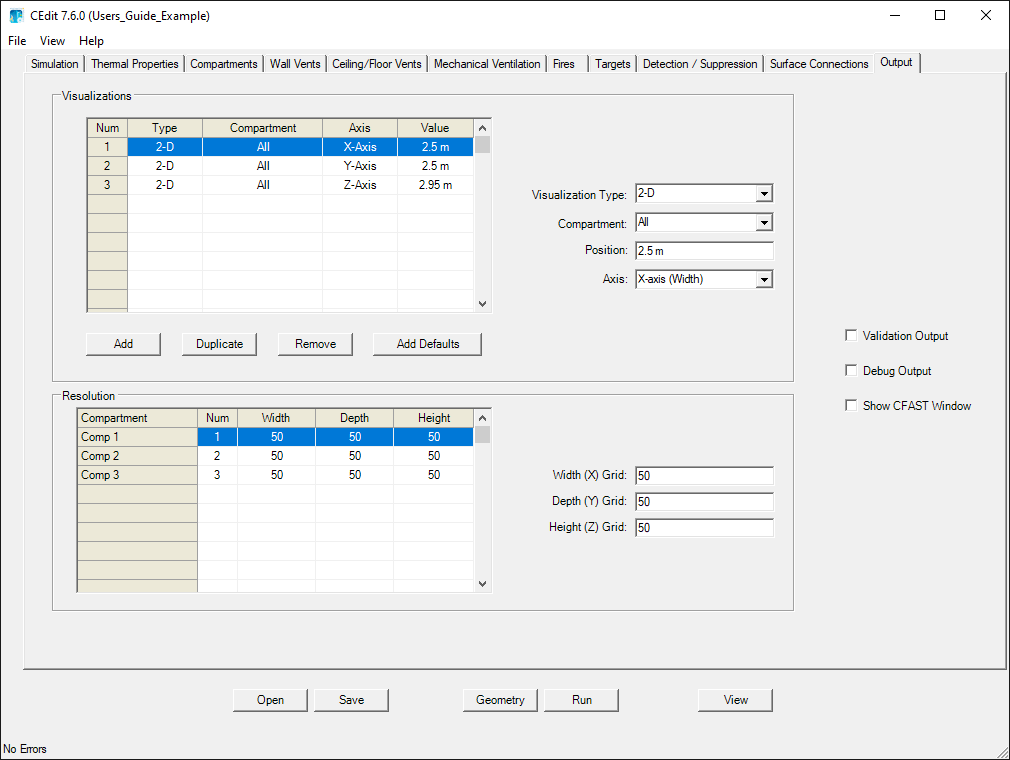
\includegraphics[width=6.5in]{FIGURES/Input_File/Visualizations_Tab}
\caption[The CFAST Visualizations Tab]{The CFAST Visualizations Tab.}
\end{center}
\end{figure}

\section{Adding Visualizations}

\begin{description}
\item[Visualization Type] (default units: n/a, default value: 2-D): The type of visualization to be included. Choose from 2-D (a single plane slice of temperature at the position and axis specified), 3-D (a set of three animated slices whose position can be moved along its respective axis, or Isosurface (a fixed 3-D surface where the gas temperature is equal to the value specified. See the Smokeview documentation \cite{Smokeview_Users_Guide_6} for details on the use of Smokeview.

\item[Compartment] (default units: n/a, default value: All): Visualizations can be placed in a single compartment or at the same position and axis in all compartments.

\item[Position] (default units: m, default value: 0m): Position along the specified axes where the slice is placed measured from the compartment origin for the selected axis (0,0,0 is the bottom left corner of the compartment. See page \pageref{Compartment_Geometry}).

\item[Axis] (default units: n/s, default value: X-axis (Width)): Axis perpendicular to the specified slice.  The slice is place perpendicular to the selected axis (the Y-Z plane for the X-Axis; the X-Z plane for the Y-Axis, and the X-Y plane for the Z-Axis)

\item[Temperature] (default units \degc, default value: none): Specified gas temperature for the selected isosurface.
\end{description}

\graybox{
Use the Add Defaults button to add a default set of visualizations for the current simulation. A slice file entry is created at the center of each compartment in the x (width) and y (depth) directions along with one near the ceiling in the z direction. A 3-D slice file entry is created for each compartment as well.
}

\section{Visualization Resolution}

By default, slice files are generated with a grid of 50 data points in each direction for each compartment specified. If desired, the grid spacing can be adjusted up or down individually by compartment. Specifying a larger number of data points can \textit{dramatically} slow program execution since the gas temperature and velocity are evaluated at each grid location every time a Smokeview output is specified.  The default value should be appropriate for most simulations.

\begin{description}
\item[Width (X) Grid] (default units: n/a, default value: 50): slices included along the X axis for each compartment are uniformly divided into the specified number of data points.

\item[Width (Y) Grid] (default units: n/a, default value: 50): slices included along the Y axis for each compartment are uniformly divided into the specified number of data points.

\item[Width (Z) Grid] (default units: n/a, default value: 50): slices included along the Z axis for each compartment are divided into the specified number of data points.
\end{description}

Sample visualizations are included below.

\begin{figure}[h!]
\begin{center}
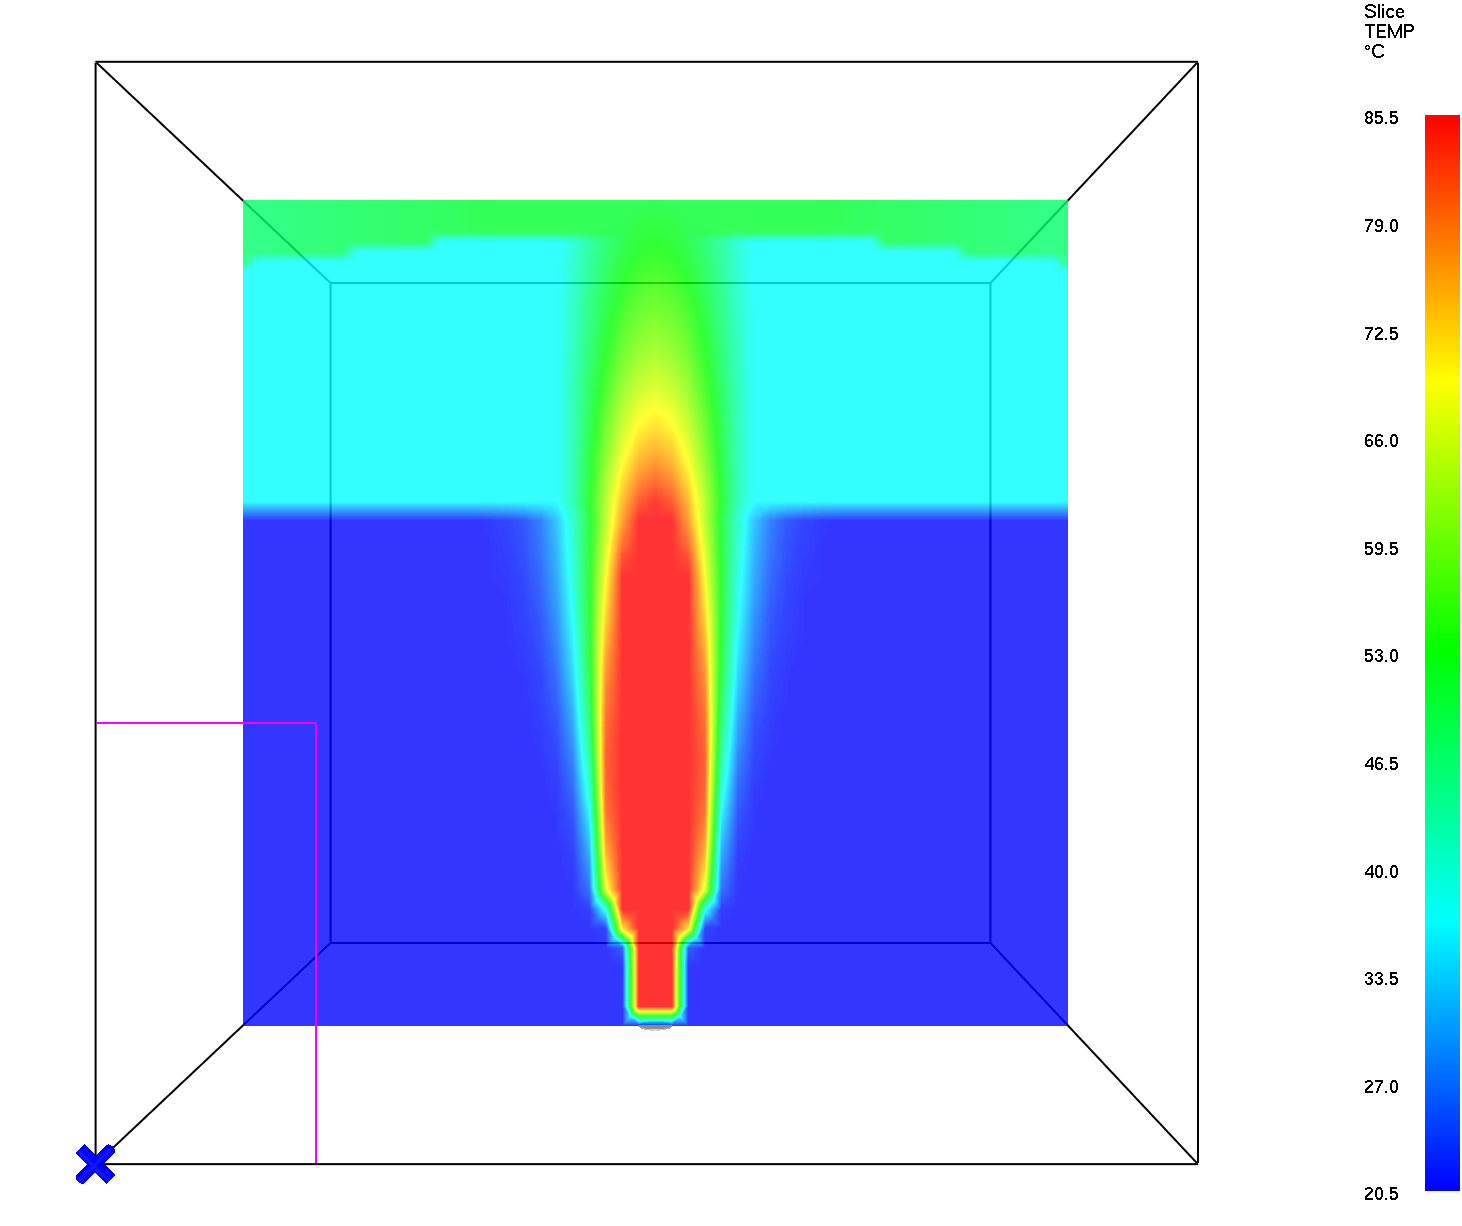
\includegraphics[width=6.5in]{FIGURES/Input_File/SMV_Temperature}
\caption{Smokeview Visualization of Gas Temperature with a Single Fire}
\end{center}
\end{figure}

\begin{figure}[h!]
\begin{center}
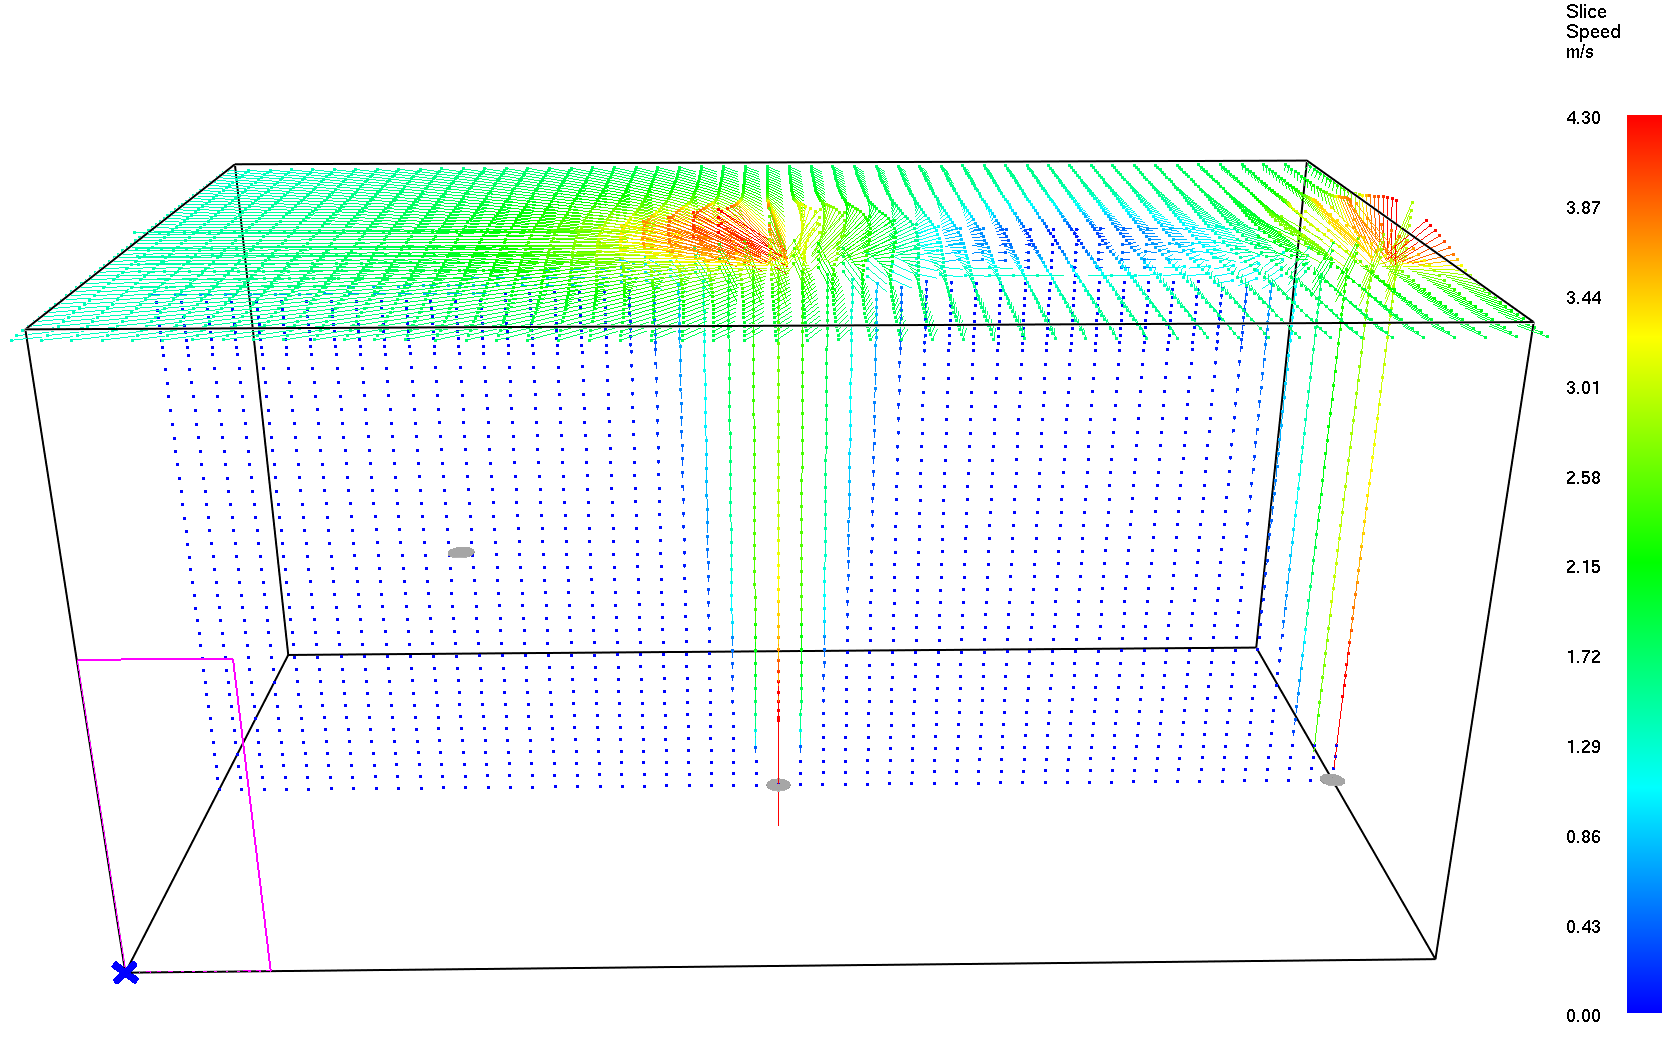
\includegraphics[width=6.5in]{FIGURES/Input_File/SMV_Velocity}
\caption{Smokeview Visualization of Gas Velocity with Two Fires}
\end{center}
\end{figure}

\begin{figure}[h!]
\begin{center}
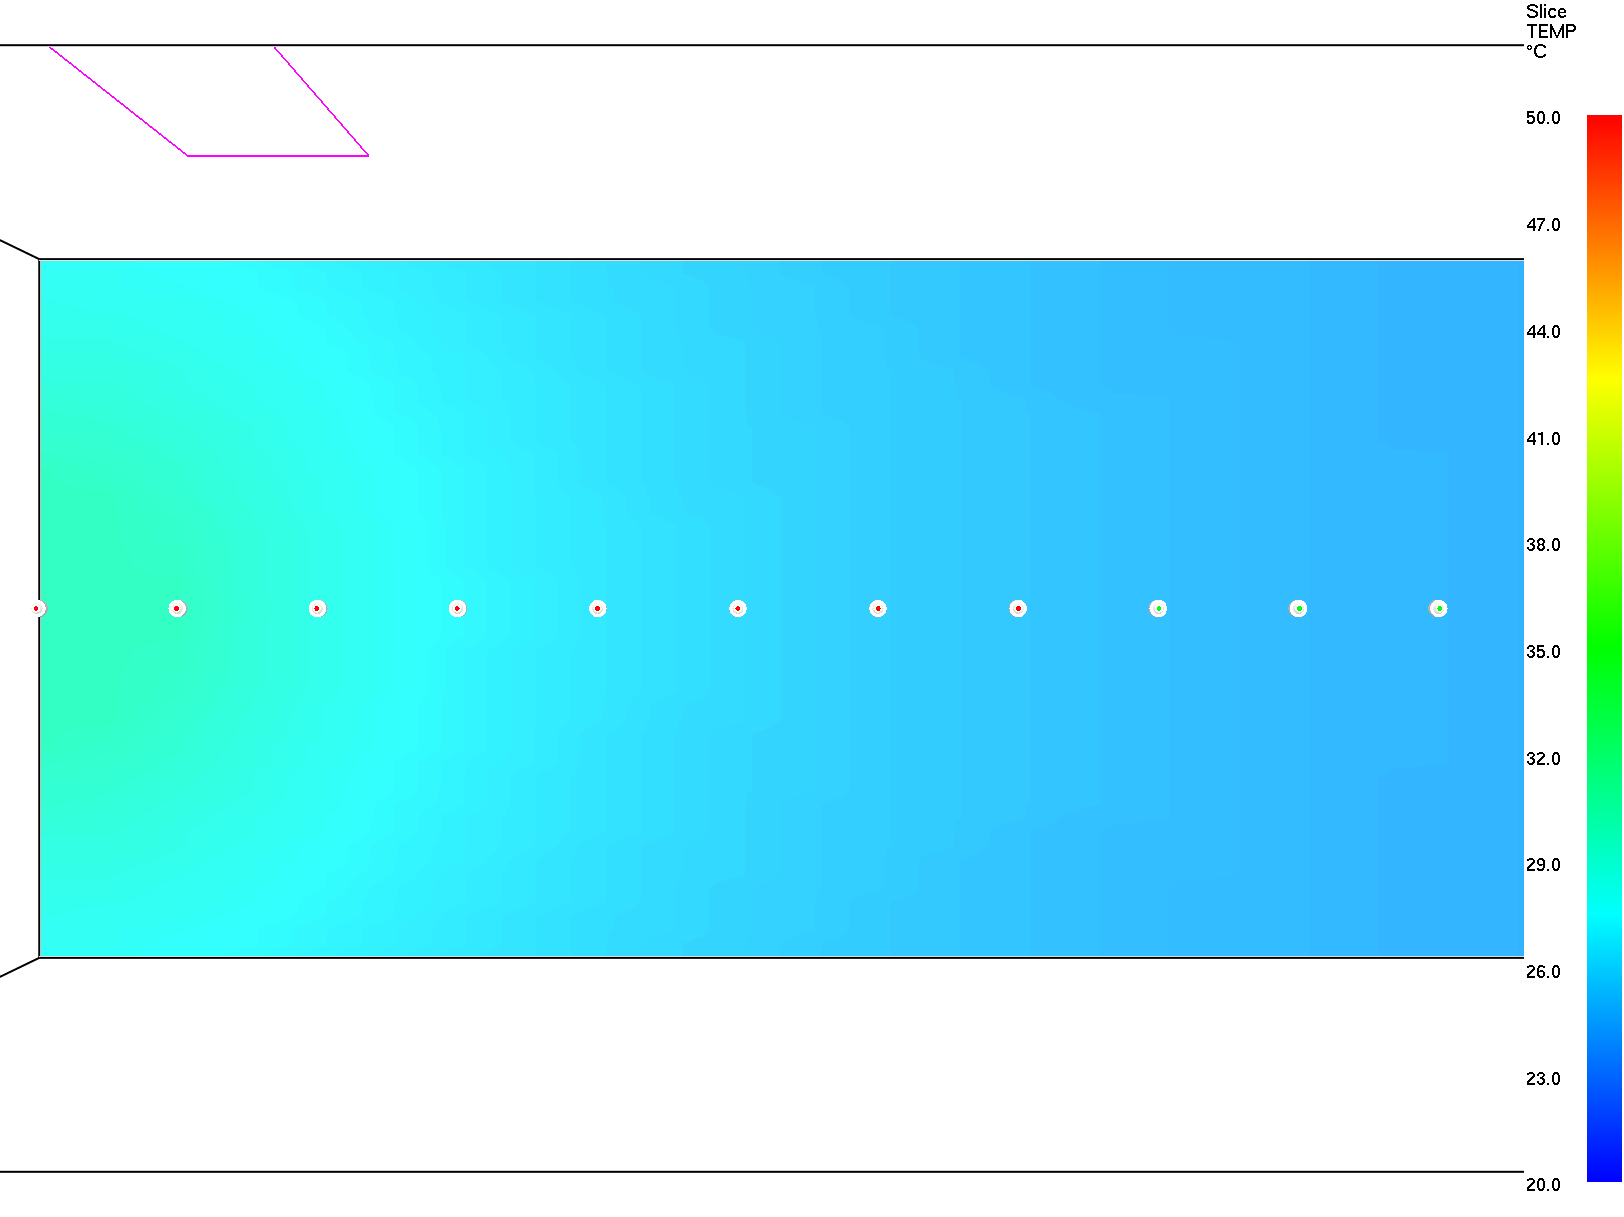
\includegraphics[width=6.5in]{FIGURES/Input_File/SMV_Detectors}
\caption{Smokeview Visualization of Detector Activation in a Corridor}
\end{center}
\end{figure}

